% Just The Docs Front Matter
% title: Modeling Jakobshavn Isbr&#230;
% parent: Tutorials
% has_children: false
% has_toc: false

\subsection{Modeling Jakobshavn Isbr\ae} \label{sec:using-issm-tutorials-jks}
\subsubsection{Goals} %{{{
\begin{itemize}
	\item Construct a 2-dimensional model of Jakobshavn Isbr\ae, West Greenland
	\item Follow a simple tutorial exercise: create and parametrize an ISSM model
	\item Use ISSM to invert for a basal friction parameter on a real-world domain
\end{itemize}

Change into \lstinlinebg|<ISSM_DIR>/examples/Jakobshavn/| to do this tutorial.
%}}}

\subsubsection{Introduction}
In this tutorial, we construct a 2-dimensional model of Jakobshavn Isbr\ae, West Greenland, and use it to invert for the basal friction parameter.

\paragraph{Download}
For this tutorial, we will use a dataset from the \href{https://scholarworks.umt.edu/cgi/viewcontent.cgi?params=/context/cs_pubs/article/1020/&path_info=Ice_sheet_model.pdf}{SeaRISE Initiative}: \lstinlinebg|Greenland_5km_v1.2.nc|. This data should be saved in the \lstinlinebg|examples/Data| directory (see 
%__@LATEX_ONLY_START@__
\hyperref[sec:using-issm-tutorials-datasets]{dataset download} section).
%__@LATEX_ONLY_END@__
%__@MARKDOWN_ONLY_START@__
% <a href="datasets">dataset download</a> page).
%__@MARKDOWN_ONLY_END@__

\subsubsection{runme file}
The \lstinlinebg|runme.m| file in \lstinlinebg|<ISSM_DIR>/examples/Jakobshavn/| is a list of commands to be run in sequence at the MATLAB command prompt. The tutorial is decomposed into 4 steps:
\begin{enumerate}
	\item Mesh generation (anisotropic adaptation)
	\item Model parameterization (using the SeaRISE dataset)
	\item Launch of the inversion for basal friction
	\item Plotting of the results
\end{enumerate}
We will follow these steps one by one by changing the selected step at the top in \lstinlinebg|runme.m|.

\subsubsection{Step 1: Mesh generation}
Open \lstinlinebg|runme.m| and make sure that the first step is activated:
\begin{lstlisting}
steps = [1];
\end{lstlisting}
In the first step, we create a triangle mesh with 2,000 meter resolution using the domain outline file \lstinlinebg|Domain.exp|. We then interpolate the observed velocity data onto the newly-created mesh. We use these observations to refine the mesh accordingly using \lstinlinebg|bamg|. In regions of fast flow we apply 1,200 m resolution, and in slow flowing areas we increase the resolution to up to 15 km:
\begin{lstlisting}
md = bamg(md, 'hmin', 1200, 'hmax', 15000, 'field', vel, 'err', 5);
\end{lstlisting}

Go to \lstinlinebg|trunk/| and launch MATLAB and then go to \lstinlinebg|examples/Jakobshavn/|:
\begin{lstlisting}
$ cd ${ISSM_DIR}
$ matlab
>> cd examples/Jakobshavn/
\end{lstlisting}

Then execute the first step:
\begin{lstlisting}
>> runme
	Step 1: Mesh creation
		  Anisotropic mesh adaptation
		  WARNING: mesh present but no geometry found. Reconstructing...
		     new number of triangles = 3017
\end{lstlisting}

\subsubsection{Step 2: Model parameterization}
In this step parameterize the model. We set for example the geometry and ice material parameters. We use the \lstinlinebg|setmask| command to define grounded and floating areas. All ice is considered grounded for now. Type \lstinlinebg|help setmask| to display documentation on how to use this command. The model is then parameterized using the \lstinlinebg|Jks.par| file. We soften the glacier's shear margins by reducing the model's ice hardness, $B$, in the area outlined by \lstinlinebg|WeakB.exp| to a factor 0.3.

Open \lstinlinebg|runme.m| and make sure that the second step is activated: \lstinlinebg|steps = [2];|
\begin{lstlisting}
>> runme
   Step 2: Parameterization
   Loading SeaRISE data from NetCDF
   Interpolating thicknesses
   Interpolating bedrock topography
   Constructing surface elevation
   Interpolating velocities
   Interpolating temperatures
   Interpolating surface mass balance
   Construct basal friction parameters
   Construct ice rheological properties
   Set other boundary conditions
      boundary conditions for stressbalance model: spc set as observed velocities
      no smb.precipitation specified: values set as zero
      no basalforcings.melting_rate specified: values set as zero
      no balancethickness.thickening_rate specified: values set as zero
\end{lstlisting}

\subsubsection{Step 3: Control method}
In the parameterization step, we applied a uniform friction coefficient of 30. Here, we use the basal friction coefficient as a control so that the modeled surface velocities match the observed ones. The mismatch between observation and modeled surface velocities is quantified by the value of a cost function. The type of cost function determines to a large degree the result of the inversion process. Different cost functions are available, type md.inversion to see a list of available cost functions:
\begin{lstlisting}
Available cost functions:
101: SurfaceAbsVelMisfit
102: SurfaceRelVelMisfit
103: SurfaceLogVelMisfit
104: SurfaceLogVxVyMisfit
105: SurfaceAverageVelMisfit
201: ThicknessAbsMisfit
501: DragCoefficientAbsGradient
502: RheologyBbarAbsGradient
503: ThicknessAbsGradient
\end{lstlisting}
Inverting for basal drag, we can use the cost functions that start with a 1. The cost functions can be combined and weighted individually:
\begin{lstlisting}
%Cost functions
md.inversion.cost_functions = [101 103];
md.inversion.cost_functions_coefficients = ones(md.mesh.numberofvertices, 2);
md.inversion.cost_functions_coefficients(:, 1) = 40;
md.inversion.cost_functions_coefficients(:, 2) = 1;
\end{lstlisting}
Our cost function is thus the sum of \lstinlinebg|`SurfaceAbsVelMisfit'|, the absolute of the velocity misfit, and \lstinlinebg|`SurfaceLogVelMisfit'|, the logarithm of the velocity misfit. We weigh the first cost function 40 times more than the latter one.

Open \lstinlinebg|runme.m|, make sure that the third step is activated (\lstinlinebg|steps = [3];|), then run \lstinlinebg|runme.m|:
\begin{lstlisting}
>> runme
	Step 3: Control method friction
		  checking model consistency
		  marshalling file Jakobshavn.bin
		  uploading input file and queueing script
		  launching solution sequence on remote cluster
		  Launching solution sequence
		  call computational core:
		     preparing initial solution

			     control method step 1/20
				  ....
\end{lstlisting}

\subsubsection{Step 4: Display results}
Here, we display the results. Open \lstinlinebg|runme.m| and make sure that step number 4 is activated. Your results should look like this:
\begin{figure}[H]
	\begin{center}
		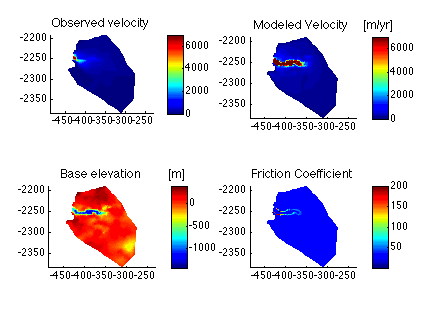
\includegraphics[width=\textwidth]{\assetsParentPath/assets/img/using-issm/tutorials/jks/JKSModel.png}
	\end{center}
\end{figure}

\clearpage % Make sure all figures are placed before next section
